\documentclass[11pt,class=report,crop=false]{standalone}
\usepackage{exo7sv}

\begin{document}

%%%%%%%%%%%%%%%%%%%%%%%%%%%%%%%%%%%%%%%%%%%%%%%%%%%%%%%%%%%%%%%%%%%%%%
%%%%%%%%%%%%%%%%%%%%%%%%%%%%%%%%%%%%%%%%%%%%%%%%%%%%%%%%%%%%%%%%%%%%%%

%%%%%%%%%%%%%%%%%%%%%%%%%%%%%%%%%%%%%%%%%%%%%%%%%%%%%%%%%%%%
\section*{\'Echauffement}

\exercice{}
\enonce
    Déterminer le domaine de définition maximal des expressions suivantes :
    \begin{examplescol}{2}
        \item $f_1(x) = x^2 +x+1$
        \item $f_2(x) = \sqrt {x-1}$
        \item $f_3(x) = \sqrt{\frac{2 + 3 x}{5-2x}}$
        \item $f_4(x) = \ln (4 x + 3)$
    \end{examplescol}
\finenonce

\indication
Pour déterminer le domaine de définition maximal des fonctions on 
doit connaître les domaines de d\'efinition des fonctions $ x \mapsto 
\tfrac{1}{x} $, $ x \mapsto \sqrt{x} $ et $ x \mapsto \ln(x) $. 
\finindication

\correction

\video{UaWs77Zaam4}

\sauteligne
\begin{enumerate}
\item 
Le domaine de d\'efinition est $ \Rr $ car la fonction $ f_1 $ est 
un polynôme. 
\item 
On sait que le domaine de d\'efinition de la fonction $ y \mapsto \sqrt{y} $ est 
$ [0, +\infty[ $. Ici, il faut que $ y = x - 1 \geq 0 $ et on obtient 
que le domaine de d\'efinition de $ f_2 $ est $ [1, +\infty[ $. 
\item 
On remarque que pour $ x = \tfrac{5}{2} $ il y aurait une division par zéro. 
Donc $ x = \tfrac{5}{2} $ ne fait pas partie du domaine de d\'efinition. 
De plus, on sait que le domaine de d\'efinition de $ y \mapsto \sqrt{y} $ 
est $ [0, +\infty[ $. Alors on doit r\'esoudre l'in\'egalit\'e $ y = 
\tfrac{2+3x}{5-2x} \geq 0 $. 
On calcule le tableau de signes :
\begin{equation*} 
\begin{tabvar}{|C|CCCCCCC|} \hline 
x    & -\infty &\hspace*{15mm}& -\frac23 &\hspace*{15mm}& \frac52 &\hspace*{15mm}& +\infty \\ \hline 
2+3x && - &\barre0& + && + & \\ \hline
5-2x && + && + &\barre0& - &\\ \hline
\frac{2+3x}{5-2x} && - && + &\dbarre& - &\\ \hline
\end{tabvar} 
\end{equation*} 

Alors le domaine de d\'efinition de $ f_3 $ est $ \left[-\frac{2}{3}, \tfrac{5}{2}\right[ $. 
\item 
On sait que le domaine de d\'efinition de $ y \mapsto \ln(y) $ est $ ]0, 
+\infty[ $. Ici, il faut que $ y = 4x + 3 > 0 $ et le domaine de d\'efinition 
de $ f_4 $ est $ \left]-\tfrac{3}{4}, +\infty\right[ $. 
\end{enumerate}
\fincorrection
\finexercice


\exercice{}
\enonce
Soit $f : x\mapsto -x^2+x+2$.
\begin{enumerate}
  \item Déterminer les racines de $f$.
  \item Dresser le tableau des variations de $f$ et donner ses intervalles de monotonie.
  \item Tracer le graphe de la fonction $f$. Donner son image.
  \item Résoudre les inégalités $f(x) \leq 0$, $f(x) > 1$, $f(x) < 5$.
\end{enumerate}
\finenonce

\indication
Utiliser la méthode de résolution des équation du second degré à l'aide du discriminant.
Pour connaître les variations de $f$ on calcule le signe de sa dérivée.
\finindication

\correction

\video{fJMT53DUGBE}

\sauteligne
\begin{enumerate}
  \item On cherche à résoudre l'équation du second degré $-x^2+x+2=0$.
  On calcule le discriminant :
  \begin{equation*}
  \Delta = 1^2 - 4 \times (-1) \times 2 = 9 > 0.
  \end{equation*}
  L'équation admet donc deux solutions :
  \begin{equation*}
  x_1 = \frac{-1 + \sqrt{9}}{2 \times (-1)} = -1 \quad \text{et} \quad x_2 = \frac{-1 - \sqrt{9}}{2 \times (-1)} = 2.
  \end{equation*}
  
  \item On calcule la dérivée de $f$ :
  \begin{equation*}
  f'(x) = -2x+1.
  \end{equation*}
  On a donc $f'(x)=0 \Leftrightarrow x=\frac12$.
  De plus $f(\frac12)=\frac94$.
  
  On en déduit le tableau de variations de $f$ :
  \begin{center}
    \begin{tikzpicture}[scale=0.8]
    % Horizontales
    % \draw(0,0) -- ++(10,0);
    \draw(0,3) -- ++(10,0); 
    \draw(0,5) -- ++(10,0); 
    
    % Verticales
    \draw(2,0) -- ++ (0,6);
    
    % Première colonne
    \node at (1,5.5) {$x$};
    \node at (1,4) {$f'(x)$};
    \node at (1,1.5) {$f(x)$};
    
    % Autres colonnes
    \node at (2.75,5.5) {$-\infty$};
    %\draw(2.45,0) -- ++ (0,5);
    %\draw(2.55,0) -- ++ (0,5);
    
    \node at (6,5.5) {$\frac12$};
    \node at (6,4) {$0$};
    \draw(6,3) -- ++ (0,2);
    
    \node at (9.25,5.5) {$+\infty$};
    
    \node[scale=1.5] at (4.25,4) {$+$};
    \node[scale=1.5] at (7.55,4) {$-$};
    
    \draw[->,>=latex,thick](2.75,0.5)--++(3,1.5);
    \draw[->,>=latex,thick](6.25,2)--++(3,-1.5);
    
    \node[scale=1] at (6,2.25) {$\frac94$};
    \end{tikzpicture}
  \end{center}
  La fonction $f$ est monotone sur les intervalles $]-\infty; \frac12]$ et sur $[\frac12; +\infty[$.
  
  \item Le graphe de $f$ est une parabole renversée de sommet $(\frac12,\frac94)$.
  Les points d'intersection avec l'axe des abscisses sont : $(-1,0)$ et $(2,0)$.
  On calcule le point d'intersection de la courbe avec l'axe des ordonnées : $(0, f(0))=(0,2)$.
  Enfin on trace le graphe :
 
  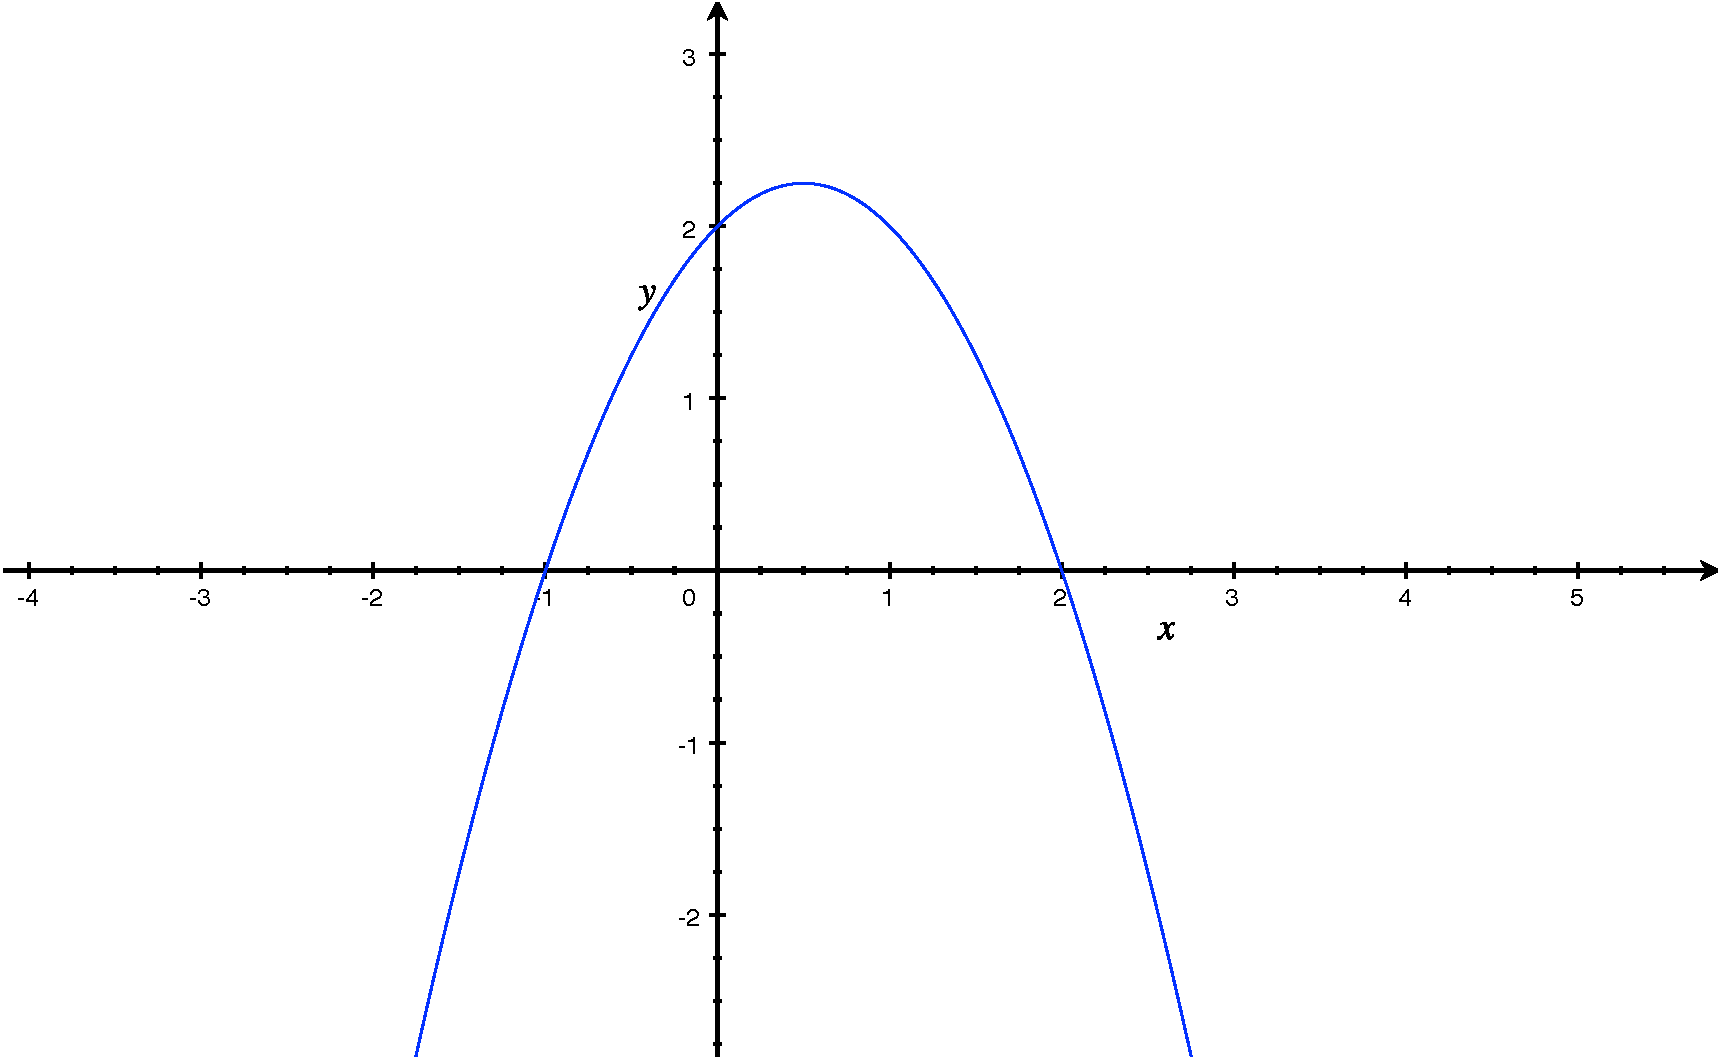
\includegraphics[width=15cm]{figures/plot_exo2}
  
  L'image de $f$ est l'intervalle $]-\infty; \frac94]$ (avec $\frac94=2,25$).
  
  \item 
  \begin{itemize}
     \item On sait que les solutions de l'équation $f(x) = 0$ sont $-1$ et $2$. En utilisant le tableau de variations de $f$ on en déduit :
  \begin{equation*}
  f(x) \leq 0 \ \Leftrightarrow \ x \in ]-\infty; -1] \text{ ou } x \in [2; +\infty[.
  \end{equation*}
     \item On résout l'équation $f(x) = 1$ dont les solutions sont $\frac{1-\sqrt5}2$ et $\frac{1+\sqrt5}2$.
  En utilisant le tableau de variation de $f$ on en déduit :
  \begin{equation*}
  f(x) > 1 \ \Leftrightarrow \ x \in ]\frac{1-\sqrt5}2; \frac{1+\sqrt5}2[.
  \end{equation*}
     \item Enfin le maximum de $f$ étant $\frac94 < 5$, on a :
  \begin{equation*}
  f(x) < 5 \text{ pour tout $x \in \mathbb{R}$}.
  \end{equation*}
  \end{itemize}
  On n'oublie pas de vérifier sur le graphe de $f$ que les résultats sont cohérents.
\end{enumerate}
\fincorrection
\finexercice




\stepcounterexo


\exercice{}
\enonce
    Résoudre les équations suivantes~:
    \begin{examplescol}{2}
        \item $3\ln \left( x+4\right) =9$
        \item $\ln \left( x+2\right) +\ln \left( x\right) =3$ 
        \item $e^{x}=e^{1-x}$
        \item $e^{3x}-2e^{-x}=0$
    \end{examplescol}
\finenonce

\indication
Pour r\'esoudre ces \'equations on remarque que la fonction $ y \mapsto 
\ln(y) $ et la fonction r\'eciproque de la fonction $ x \mapsto e^{x} $, 
c'est-\`a-dire $ y = e^{x} $ si et seulement si $ x = \ln(y) $. 
\finindication

\correction

\video{VK-pJKmxKBs}

\sauteligne
\begin{enumerate}
\item 
$ 
3 \ln\left(x + 4\right) = 9 \Longleftrightarrow \ln\left(x + 4\right) = 3 
\Longleftrightarrow x + 4 = e^3 \Longleftrightarrow x = e^3 - 4 
$. 
\item 
$ 
\ln\left(x + 2\right) + \ln\left(x\right) = 3 \Longrightarrow 
\ln\left(x(x+2)\right) = 3 \Longrightarrow x(x+2) = e^3 \Longrightarrow 
x^2 + 2x - e^3 = 0 \Longrightarrow $ $ x = -1 + \sqrt{e^3 + 1} 
\ \text{ou}\ x = -1 - \sqrt{e^3 + 1} $. 
Mais attention, dans l'équation initiale $x$ doit être strictement positif. Il ne reste qu'une seule solution valide c'est $x = -1 + \sqrt{e^3 + 1}$.
\item 
$ e^{x} = e^{1-x} \Longleftrightarrow \ln\left(e^{x}\right) = \ln\left(e^{1-x}\right) 
\Longrightarrow x = 1 - x \Longleftrightarrow 2x = 1 \Longleftrightarrow x = \tfrac{1}{2} $. 
\item 
$ e^{3x} - 2e^{-x} = 0 \Longleftrightarrow e^{3x} = 2 e^{-x} \Longleftrightarrow 
\ln\left(e^{3x}\right) = \ln\left(2 e^{-x}\right) \Longleftrightarrow 3x = \ln(2) 
+ \ln\left(e^{-x}\right) \Longleftrightarrow 3x = \ln(2) - x \Longleftrightarrow 
4x = \ln(2) \Longleftrightarrow x = \tfrac{\ln(2)}{4} $. 
\end{enumerate} 
\fincorrection 
\finexercice

\exercice{}
\enonce
  Calculer les limites suivantes.
    \begin{examplescol}{3}
        \item $\displaystyle \underset{x \to +\infty}{\lim} \frac{e^{x}}{x}$
        \item $\displaystyle \underset{x \to 1}{\lim} \frac{x-1}{\ln(x)} $
        \item $\displaystyle \underset{x \to +\infty}{\lim} \frac{x^{2}+3}{2x^{2}+x+1} $
        \item $\displaystyle \underset{x \to 0}{\lim} \frac{\sin(x)}{x} $
        \item $\displaystyle \underset{x \to +\infty}{\lim} \sqrt{x^{2}-x}-x $
        \item[]
    \end{examplescol}  
\finenonce

\indication
Pour a), on se rappellera des théorèmes de croissances comparées.
Pour b) et d), il faut utiliser la définition de la dérivée comme limite du taux d'accroissement.
Pour c), il faut mettre en facteur les termes dominants du numérateur et du dénominateur.
Pour e), il faut faire apparaître la \og quantité conjuguée \fg{} : $\sqrt{x^{2}-x}+x$.
\finindication

\correction

\video{74pEWPSSSQ0}

\sauteligne
\begin{enumerate}
  \item Par croissances comparées on a
  \begin{equation*}
  \lim_{x \to +\infty} \frac{e^{x}}{x} = +\infty.
  \end{equation*}
  
  \item On fait apparaître la limite du taux d'accroissement de $\ln$ en $x=1$ :
  \begin{equation*}
  \lim_{x \to 1} \frac{\ln(x)}{x-1} = \lim_{x \to 1} \frac{\ln(x) - \ln(1)}{x-1}  = \ln'(1) = 1.
  \end{equation*}
  Ainsi $\lim_{x \to 1} \frac{x-1}{\ln(x)} = 1$.
  
  \item On met en facteur les termes dominants du numérateur et du dénominateur :
  \begin{equation*}
  \lim_{x \to +\infty} \frac{x^{2}+3}{2x^{2}+x+1} = \lim_{x \to +\infty} \frac{x^{2}(1+\frac3{x^2})}{x^{2}(2+\frac1x+\frac1{x^2})} = \lim_{x \to +\infty} \frac{1+\frac3{x^2}}{2+\frac1x+\frac1{x^2}} = \frac12.
  \end{equation*}
  
  \item On fait apparaître la limite du taux d'accroissement de $\sin$ en $x=0$ :
  \begin{equation*}
  \lim_{x \to 0} \frac{\sin(x)}{x} = \lim_{x \to 0} \frac{\sin(x)-\sin(0)}{x-0} = \sin'(0) = \cos(0) = 1.
  \end{equation*}
  
  \item On fait apparaître la quantité conjuguée :
  \begin{align*}
  \lim_{x \to +\infty} \sqrt{x^{2}-x}-x &= \lim_{x \to +\infty} \frac{(\sqrt{x^{2}-x}-x)(\sqrt{x^{2}-x}+x)}{\sqrt{x^{2}-x}+x} \\
  &= \lim_{x \to +\infty} \frac{(x^{2}-x)-x^2}{\sqrt{x^{2}-x}+x} \\
  &= \lim_{x \to +\infty} \frac{-x}{x\sqrt{1-\frac1x}+x} \\
  &= \lim_{x \to +\infty} \frac{-1}{\sqrt{1-\frac1x}+1} \\
  &= -\frac12.
  \end{align*}
\end{enumerate}
\fincorrection
\finexercice


\exercice{}
\enonce
    Étudier les fonctions suivantes.

    \begin{examplescol}{3}
        \item $\displaystyle \frac{x^{2}-x-2}{x-3} $
        \item $\displaystyle \sqrt{\frac{x+1}{x+2}} $
        \item $\displaystyle \ln\left(x-\frac{1}{x}\right) $
    \end{examplescol}
\finenonce

\indication
Pour étudier une fonction $ f(x) $ il faut donner le domaine de d\'efinition, 
les asymptotes \'eventuelles, dériver la fonction $ f(x) $ et étudier le signe 
de $ f'(x) $.
\finindication

\correction

\video{YAOOPnAFcyg}

\video{iL4j52FINR0}

\video{78UwZ4I1CRQ}

\sauteligne
\begin{enumerate}
\item 
Soit $ f(x) = \tfrac{x^{2}-x-2}{x-3} $. Le domaine de définition est $ \Rr \setminus 
\{3\}$, car pour $ x = 3 $ il y aurait une division par zéro. Le comportement de $ f $ 
aux bord de son domaine de d\'efinition est 
\begin{align*} 
\lim_{x \rightarrow -\infty} f(x) = \lim_{x \rightarrow -\infty} \frac{x^2}{x} 
= \lim_{x \rightarrow -\infty} x = -\infty,  
\qquad & \qquad 
\lim_{x \rightarrow +\infty} f(x) = \lim_{x \rightarrow +\infty} \frac{x^2}{x} 
= \lim_{x \rightarrow +\infty} x = +\infty, \\ 
\lim_{x \rightarrow 3^{-}} f(x) = -\infty \ \left(\text{ en tant que }\flqq \frac{4}{0^{-}}\frqq\right), 
\qquad & \qquad 
\lim_{x \rightarrow 3^{+}} f(x) = +\infty \ \left(\text{ en tant que }\flqq\frac{4}{0^{+}}\frqq\right). 
\end{align*}
Alors il y a une asymptote verticale d'\'equation $ x = 3 $ et des asymptotes 
obliques de l'\'equation $ ax + b $ en $ \pm \infty $. Pour d\'eterminer $ a $ et 
$ b $ on calcule 
\begin{equation*} 
a = \lim_{x \rightarrow \pm\infty} \frac{f(x)}{x} = 
\lim_{x \rightarrow \pm\infty} \frac{x^2}{x^2} = 1 
\end{equation*} 
et 
\begin{equation*} 
b = \lim_{x \rightarrow \pm\infty} f(x) - ax 
= \lim_{x \rightarrow \pm\infty} \frac{x^{2}-x-2}{x-3} - x 
= \lim_{x \rightarrow \pm\infty} \frac{2x-2}{x-3} 
= \lim_{x \rightarrow \pm\infty} \frac{2x}{x} 
= 2. 
\end{equation*} 
On remarque qu'on a le m\^eme calcul pour $ +\infty $ et $ -\infty $. Maintenant on 
\'etudie les variations de $ f $~: 
\begin{equation*} 
f'(x) = \frac{(2x-1)(x-3) - (x^2-x-2)}{(x-3)^2} = \frac{x^2 - 6x + 5}{(x-3)^2} 
= \frac{(x - 1)(x -5)}{(x-3)^2}
\end{equation*} 
Alors 
\begin{equation*} 
\begin{tabvar}{|C|CCCCCCCCCCC|} \hline 
x & -\infty && 1 &&& 3 &&& 5 && +\infty \\ \hline 
(x - 3)^2 &&&&&&& + &&&& \\ \hline 
x - 1 && - & \barre0 &&&& + &&&& \\ \hline 
x - 5 &&&& - &&&&& \barre0 & + & \\ \hline 
f'(x) && + & \barre0 & - && \dbarre && - & \barre0 & + & \\ \hline 
\niveau{1}{3} \TVcenter{f(x)} & 
-\infty & \croit & \text{max} & \decroit & -\infty & \dbarre & 
\niveau{3}{3} +\infty & \decroit & \text{min} & \croit & +\infty \\ \hline 
\end{tabvar} 
\end{equation*} 
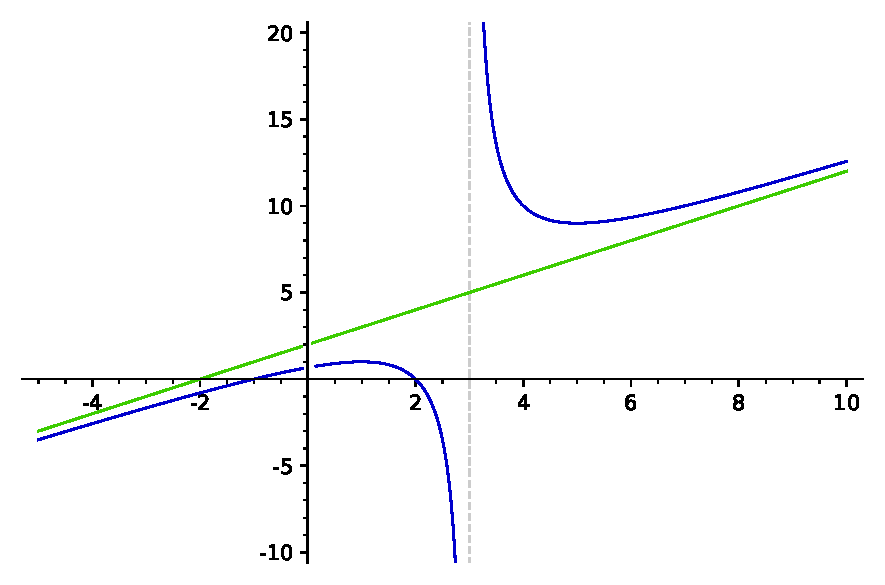
\includegraphics{figures/plot1} 
\item 
Soit $ f(x) = \sqrt{\tfrac{x+1}{x+2}} $. 
On sait que $ x + 2 = 0 $ si et seulement si $ x = -2 $. Donc $ -2 $ 
n'appartient pas au domaine de d\'efinition de $ f $.

Le domaine de définition de la fonction 
$ y \mapsto \sqrt{y} $ est $ [0, +\infty[ $. 
On étudie le signe de $y=\frac{x+1}{x+2}$ à l'aide d'un tableau :
\begin{equation*} 
\begin{tabvar}{|C|CCCCCCC|} \hline 
x    & -\infty &\hspace*{15mm}& -2 &\hspace*{15mm}& -1 &\hspace*{15mm}& +\infty \\ \hline 
x+1 && - && - &\barre0& + & \\ \hline
x+2 && - &\barre0& + && + &\\ \hline
\frac{x+1}{x+2} && + &\dbarre& - &\barre0& + &\\ \hline
\end{tabvar} 
\end{equation*} 

Il faut que $ y = \tfrac{x+1}{x+2} 
\geq 0 $.  Alors le domaine de d\'efinition de $ f $ est $ ]-\infty, -2[ \ 
\cup \ [-1, +\infty[ $. Le comportement de $ f $ aux bord de son domaine de d\'efinition 
est 
\begin{align*} 
\lim_{x \rightarrow -\infty} f(x) = \lim_{x \rightarrow -\infty} \sqrt{\frac{x}{x}} 
= \lim_{x \rightarrow -\infty} 1 = 1,  
\qquad & \qquad 
\lim_{x \rightarrow +\infty} f(x) = \lim_{x \rightarrow +\infty} \sqrt{\frac{x}{x}} 
= \lim_{x \rightarrow +\infty} 1 = 1, \\ 
\lim_{x \rightarrow -2^{-}} f(x) = +\infty \ \left(\text{ en tant que }\flqq \frac{-1}{0^{-}}\frqq\right), 
\qquad & \qquad 
\lim_{x \rightarrow -1^{+}} f(x) = f(-1) = 0. 
\end{align*}
Alors il y a une asymptote verticale d'\'equation $ x = -2 $ et une asymptote horizontale 
d'\'equation $ y = 1 $. Maintenant on \'etudie les variations de $ f $~: 
\begin{equation*} 
f'(x) = \frac{1}{2 \sqrt{\tfrac{x+1}{x+2}}} \left(\frac{x+1}{x+2}\right)'
= \frac{1}{2 \sqrt{\tfrac{x+1}{x+2}}} \frac{x+2-(x+1)}{(x+2)^2} 
= \frac{1}{2 \sqrt{\tfrac{x+1}{x+2}}} \frac{1}{(x+2)^2} 
\end{equation*} 
Alors 
\begin{equation*} 
\begin{tabvar}{|C|CCCRULCC|} \hline 
x & -\infty &&& -2 & \hspace*{15mm} & -1 &&  +\infty \\ \hline 
f'(x) && + && \dbarre &&& + &  \\ \hline 
\niveau{1}{2} \TVcenter{f(x)} & 
1 & \croit & +\infty & \dbarre & & 
\niveau{1}{2} 0 & \croit & 1 \\ \hline 
\end{tabvar} 
\end{equation*} 
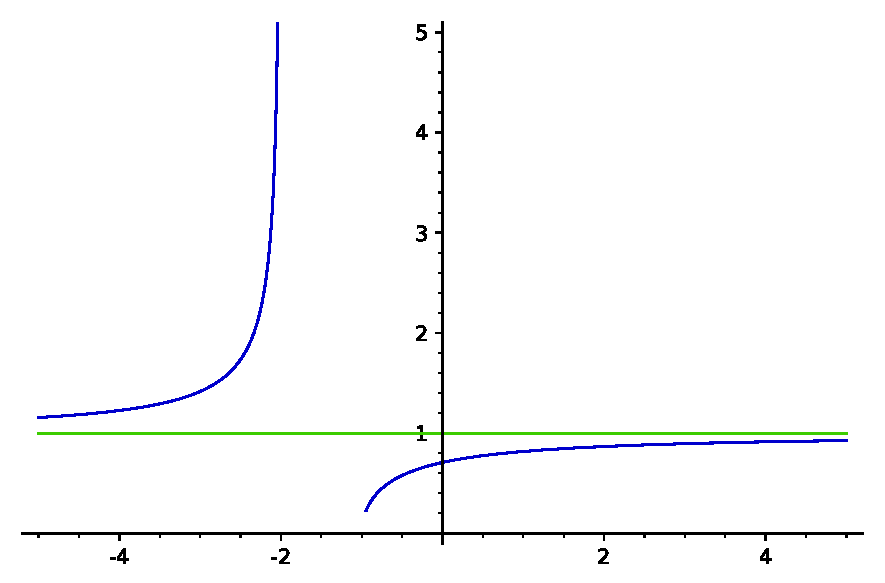
\includegraphics{figures/plot2} 
\item 
Soit $ f(x) = \ln\left(x - \tfrac{1}{x}\right) $. Le domaine de définition 
de la fonction $ y \mapsto \ln(y) $ est $ ]0, +\infty[ $. Alors il faut que 
$ y = x - \tfrac{1}{x} > 0 $. On étudie le signe de $x-\frac1x = \frac{x^2-1}{x} = \frac{(x-1)(x+1)}{x}$.

\begin{equation*} 
\begin{tabvar}{|C|CCCCCCCCC|} \hline 
x    & -\infty &\hspace*{15mm}& -1 &\hspace*{15mm}& 0 &\hspace*{15mm}&+1 &\hspace*{15mm}& +\infty \\ \hline 
x-1 && - && - && - &\barre0& + & \\ \hline
x+1 && - &\barre0& + && + && + & \\ \hline
x && - && - &\barre0& + && + &\\ \hline
\frac{(x-1)(x+1)}{x} && - &\barre0& + &\dbarre& - &\barre0&+&\\ \hline
\end{tabvar} 
\end{equation*} 

Finalement, on obtient que le domaine de d\'efinition de $ f $ est $ ]-1; 0[ 
\ \cup \  ]1; +\infty[ $. Le comportement de $ f $ aux bords de son domaine de 
d\'efinition est 
\begin{align*} 
\lim_{x \rightarrow -1^{+}} f(x) = \lim_{x \rightarrow 0^{+}} \ln(x) = 
-\infty,  
\qquad & \qquad 
\lim_{x \rightarrow 0^{-}} f(x) = \lim_{x \rightarrow +\infty} \ln(x) = 
+\infty, \\ 
\lim_{x \rightarrow 1^{+}} f(x) = \lim_{x \rightarrow 0^{+}} \ln(x) = 
-\infty, 
\qquad & \qquad 
\lim_{x \rightarrow +\infty} f(x) = \lim_{x \rightarrow +\infty} \ln(x) = 
+\infty. 
\end{align*} 
Alors il y a des asymptotes verticales d'\'equation $ x = -1 $, $ x = 0 $ 
et $ x = 1 $. Maintenant on \'etudie les variations de $ f $~: 
\begin{equation*} 
f'(x) = \frac{1}{x - \frac{1}{x}} \left(x - \frac{1}{x}\right)' 
= \frac{1}{x - \frac{1}{x}} \left(1 + \frac{1}{x^2}\right) 
= \frac{1}{x - \frac{1}{x}} \frac{x^2 + 1}{x^2}. 
\end{equation*} 
Comme $\frac{x^2 + 1}{x^2} \ge 0$ alors $f'(x)$ est du signe de $y=x-\frac1x$ qui est positif sur le domaine de définition. Ainsi $f'(x)\ge0$ pour tout $x$ appartenant au domaine de définition.

Alors 
\begin{equation*} 
\begin{tabvar}{|C|CCCCRULCCC|} \hline 
x     & -1 &&&& 0 & \hspace*{15mm} & 1 &&&  +\infty \\ \hline 
f'(x) &&& + &&&&&& + & \\ \hline 
\niveau{1}{2} \TVcenter{f(x)} & 
\dbarre & -\infty & \croit & +\infty & \dbarre & & 
\dbarre & \niveau{1}{2} -\infty & \croit & +\infty \\ \hline 
\end{tabvar} 
\end{equation*} 
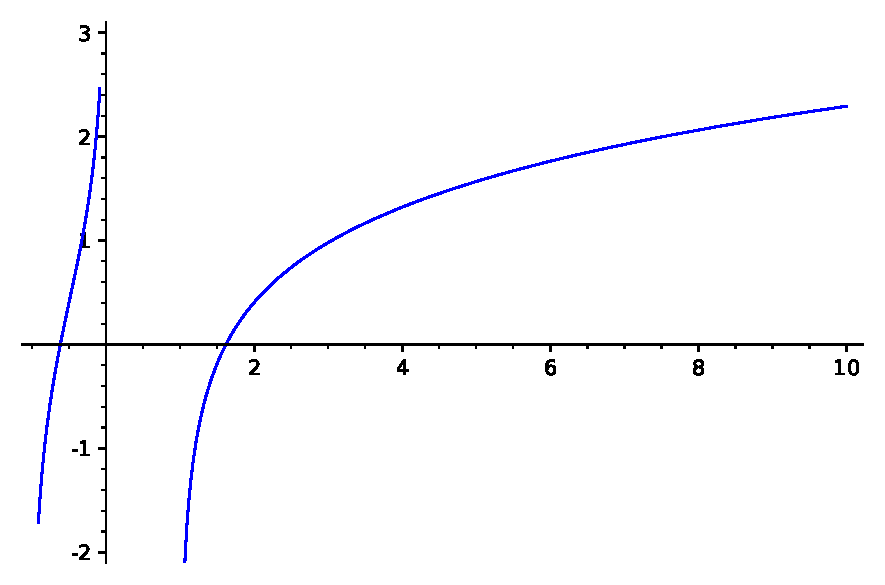
\includegraphics{figures/plot3} 
\end{enumerate} 
\fincorrection 
\finexercice



\end{document}